\chapter{802.15.4 Application}

\section{Fabric Architecture}
802.15.4 application integrates the basic transceiver functionality into Fabric. 
User can initiate transmission or receiving by simply writing to specific registers.
Figure~\ref{fig:radio_state} is a simplified model of state machine. The details for each state
will be discussed in following.
\begin{figure}[t]
	\centering
	
\includegraphics[width=0.6\columnwidth]{radio_state}
	\caption{Simplified radio state diagram}
	\label{fig:radio_state}
\end{figure}

\begin{figure}[h]
\centering
	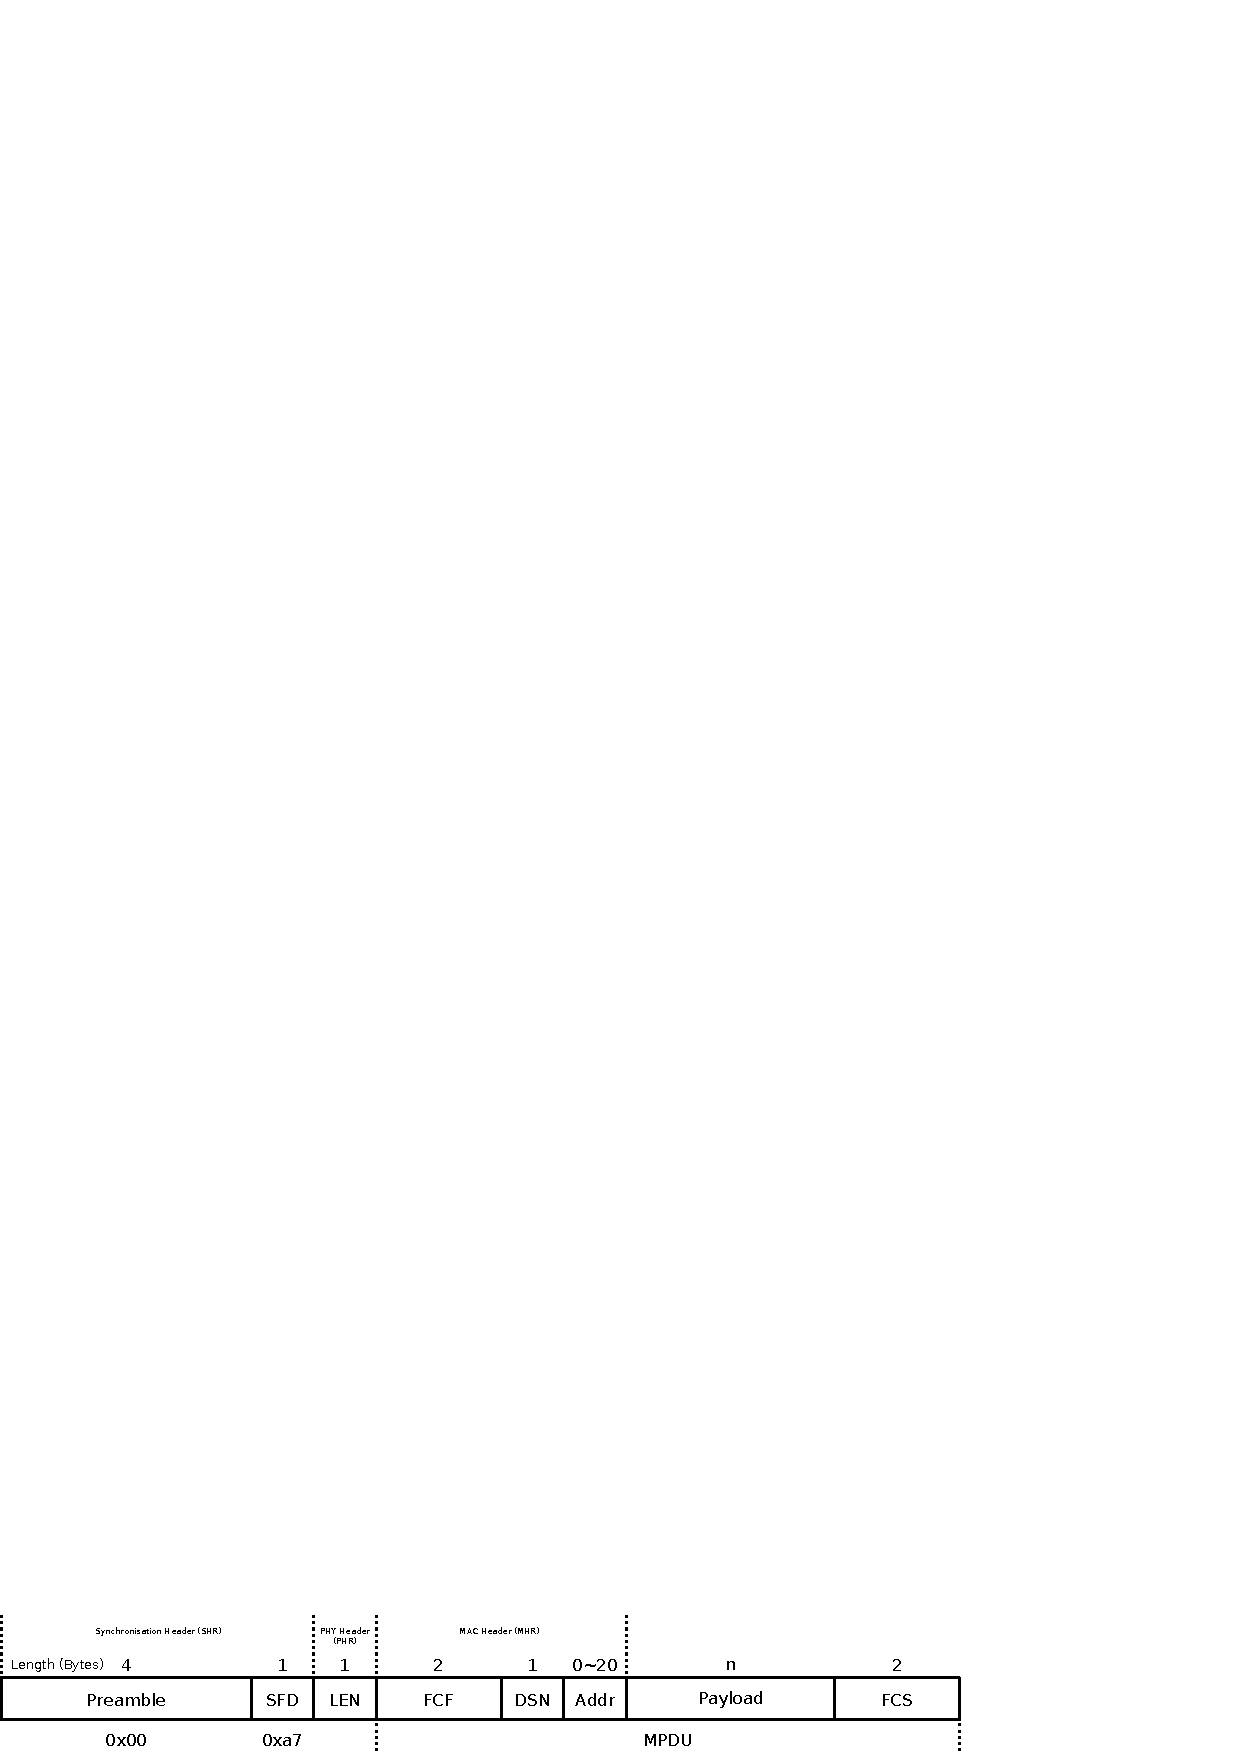
\includegraphics[width=0.9\columnwidth]{frame_format}
	\caption{Frame format of a 802.15.4 packet}
\end{figure}

\subsection{Radio states}
\subsubsection{Off Mode}
\hangindent=\parindent
\hangafter=0
Once the \sdr exits global system reset, radio starts with {\bf Off} state.
In this state, the radio peripherals (RF frontend, ADCs and DAC) are in the 
lowest power state to save energy. Radio exits this state if the following event
has been triggered.
\begin{description}
	\item[1. Deasserting Radio off/on register:] Radio exits {\bf Off} mode
	and a series of hardware initializations take place at this stage. Once the
	discrete chips are ready, the radio arrives {\bf Idle Listening} mode.
\end{description}

\subsubsection{Idle Listening Mode}
\hangindent=\parindent
\hangafter=0
In this mode, radio has RF frontend on in RX mode and ADCs actively running. Radio keeps
decoding wireless signal and trying to identify any incoming packet. In addition, radio
is ready to initiate a packet transmission in this state. Radio exits this state if the 
following event has been triggered.
\begin{description}
	\item[1. Asserting Radio off/on register] Radio turns-off all peripherals and 
	entering the {\bf Off} mode to save energy.
	\item[2. Incoming packet detected] Once a valid length field has been decoded, 
	radio enters {\bf Receiving} mode to ensure receiving a completed packet.
	\item[3. Initiating packet transmission] The start transmission command from processor
	or Fabric itself trigger the radio into {\bf Transmission} mode.
\end{description}

\subsubsection{Receiving Mode}
\hangindent=\parindent
\hangafter=0
Since the radio is not transmitting in this state, DAC has been turned-off to save energy.
In the mean time, RF frontend and ADCs actively running and receiver blocks decode
wireless data. Receiver performs a basic frame filtering and storing the incoming bytes
into fifos. Radio exits this state if the following event has been triggered.
\begin{description}
	\item[1. Receiving completed] A packet has been received completely and this packet
	doesn't request ACK nor Forward. Radio backs to {\bf Idle Listening}.
	\item[2. ACK/Foward completed] Radio backs to {\bf Idle Listening} if ACK/Forward\footnote{
	802.15.4 standard requires 192~$\mu$s between transmissions (ACK/Forward). The 
	timing requirement is taken care in hardware.}
	packet has been transmitted completed.
\end{description}

\subsubsection{Transmission Mode}
\hangindent=\parindent
\hangafter=0
In transmission mode, ADCs has been turned-off and the receiver is put into reset. Transmitter
starts reading the data from TX fifo and up converting through RF frontend. Radio exits this 
state if the following event has been triggered.
\begin{description}
	\item[1. Transmission completed] The TX fifo is empty indicates the transmission
	has been completed. Radio switches back to RX and going to {\bf Idle Listening}.
\end{description}

\clearpage
\subsection{fifos}
\sdr takes the advantage of high speed interconnect between processor and FPGA fabric. The processor
loads/unloads the data from radio by accessing to specific addresses. The writing/reading 
operation is mapped to the fifo operation. With integrated PDMA, data operation can be even
faster and requests less processor's resources.
The following fifos can be found in 802.15.4 application.
\begin{enumerate}
	\item {\bf RX fifo}
	\item {\bf TX fifo}
	\item {\bf ACK fifo}
	\item {\bf FWD fifo}
\end{enumerate}

\subsubsection{RX fifo}
\hangindent=\parindent
\hangafter=0
The depth and width of RX fifo is 512 and 8-bits respectively, which is able to store 4 packets
in maximum length. Unlike other fifos, RX fifo is an embedded fifo, whereas other fifos are
synthesized "soft" fifos.

\hangindent=\parindent
\hangafter=0
A typical 802.15.4 packet starts with 4 bytes of preamble (0x00), 1 byte of SFD (0xa7) and length
field comes after SFD. Once a valid length field has been detected, receiver start storing the
decoded byte into RX fifo until the packet ends. The last 2 bytes in the packet are FCS (Frame 
Check Sequence) field. These bytes are used to perform CRC (Cyclic Redundancy Check) to detect
errors. However, FCS is not useful to processor. Since the CRC is embedded in fabric. Instead of
storing the FCS field in RX fifo, receiver stors the averaged~\footnote{The value is averaged 
over 4 RSSI samples right before SFD has been detected. Approximately 5~$\mu$s.}
RSSI value and CRC result. 
\begin{figure}[h]
	\centering
	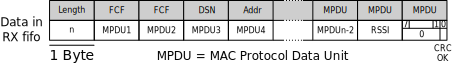
\includegraphics[width=0.6\columnwidth]{rx_fifo_content}
	\caption{The contents of RX fifo}
	\label{fig:rx_fifo_content}
\end{figure}


\hangindent=\parindent
\hangafter=0
Figure~\ref{fig:rx_fifo_content} shows the contents stored in RX fifo. The last two bytes
stored in the RX fifo are RSSI and CRC OK respectively. The RSSI value is unsigned 8 bytes
value. As mentioned before, the step size of RSSI is 14.8~mV. (eg: 137 = 2.03~V in RSSI)
CRC OK is a single bit in last byte. This bit is asserted if the packet passed CRC check
and vice versa.

\subsubsection{TX fifo}
\hangindent=\parindent
\hangafter=0
The depth and width of TX fifo is 128 and 8-bits respectively. In contrast to RX fifo, 
TX fifo contains only 1 packet every time. Transmitter loads preamble
and SFD automatically, which occupy 5 bytes in depth. Thus, the truly available depth for
user is $128 - 5 - 1$ (length) $= 122$ bytes. User only loads the "data" to TX fifo. The 
transmitter will automatically calculate corresponding FCS and appending it to the end
of TX fifo. 

\subsubsection{ACK fifo}
\hangindent=\parindent
\hangafter=0
\sdr support hardware ACK (HACK). Parts of ACK frame is pre-stored in ACK fifo. Once the received packet
has ACK request bit set, its DSN is passed to ACK fifo and fifo control starts calculating the FCS
for ACK frame. User cannot access to ACK fifo directly.

\subsubsection{FWD fifo}
\hangindent=\parindent
\hangafter=0
\sdr supports hardware packet forwarding. Receiver stores the decoded data into 2 different fifos - 
RX fifo and FWD fifo. However, the data stored in these fifos are slightly different in DSN field
and FCS. \sdr uses DSN as a relay counter to prevent the forwarding packet last forever in the network.
Only the packet has DSN which is less than threshold (0x7f) will be forwarded. Similar to TX fifo,
FWD fifo is not able to be accessed by user.

\clearpage
\subsection{Address Map}
\begin{table*}[h]
\centering
\begin{threeparttable}
	\begin{tabular}{|c|c|c|c|c|}
		\hline
		{\bf Address} & {\bf Width} & {\bf Bit Position} & {\bf Direction} & {\bf Registers} \\ \hline
		0x40050000 & 8  & 7:0 	& R		& RX fifo\\ \hline
		0x40050004 & 16 & 31:16 & R		& Src Pan ID\tnote{a}\\
		0x40050004 & 16 & 15:0	& R		& Dest Pan ID\tnote{a}\\ \hline
		0x4005000c & 1	& 18	& R		& RX fifo empty\\
		0x4005000c & 1	& 17	& R		& ACK set\tnote{a}\\
		0x4005000c & 1	& 16	& R		& CRC correct\tnote{a}\\
		0x4005000c & 16 & 15:0	& R		& FCF\tnote{a}\\ \hline
		0x40050010 & 32 & 31:0	& R		& Src address LSB\tnote{a}\\ \hline
		0x40050014 & 32 & 31:0	& R		& Src address MSB\tnote{a}\\ \hline
		0x40050018 & 32 & 31:0	& R		& Dest address LSB\tnote{a}\\ \hline
		0x4005001c & 32 & 31:0	& R		& Dest address MSB\tnote{a}\\ \hline\hline
		0x40060000 & 8	& 7:0	& W		& TX fifo\\ \hline\hline
		0x40070000 & 1	& 8		& R/W	& Auto TX en\\
		0x40070000 & 4	& 7:4	& R		& Radio mode\\
		0x40070000 & 1	& 3		& R/W	& ACK en\\
		0x40070000 & 2	& 2:1	& R/W	& AGC mode\\
		0x40070000 & 1	& 0		& R/W	& Radio off/on\\ \hline
		0x40070020 & 8	& 7:0	& R/W	& LED\\ \hline
		0x40070050 & 1	& 0		& W		& ACK flush\\ \hline\hline
		0x40080000 & 14	& 13:0	& W		& MAX2831 Register 0\tnote{b}\\ \hline
		0x40080004 & 14	& 13:0	& W		& MAX2831 Register 1\tnote{b}\\ \hline
		0x40080008 & 14	& 13:0	& W		& MAX2831 Register 2\tnote{b}\\ \hline
		0x4008000c & 14	& 13:0	& W		& MAX2831 Register 3\tnote{b}\\ \hline
		0x40080010 & 14	& 13:0	& W		& MAX2831 Register 4\tnote{b}\\ \hline
		0x40080014 & 14	& 13:0	& W		& MAX2831 Register 5\tnote{b}\\ \hline
		0x40080018 & 14	& 13:0	& W		& MAX2831 Register 6\tnote{b}\\ \hline
		0x4008001c & 14	& 13:0	& W		& MAX2831 Register 7\tnote{b}\\ \hline
		0x40080020 & 14	& 13:0	& W		& MAX2831 Register 8\tnote{b}\\ \hline
		0x40080024 & 14	& 13:0	& W		& MAX2831 Register 9\tnote{b}\\ \hline
		0x40080028 & 14	& 13:0	& W		& MAX2831 Register 10\tnote{b}\\ \hline
		0x4008002c & 14	& 13:0	& W		& MAX2831 Register 11\tnote{b}\\ \hline
		0x40080030 & 14	& 13:0	& W		& MAX2831 Register 12\tnote{b}\\ \hline
		0x40080034 & 14	& 13:0	& W		& MAX2831 Register 13\tnote{b}\\ \hline
		0x40080038 & 14	& 13:0	& W		& MAX2831 Register 14\tnote{b}\\ \hline
		0x4008003c & 14	& 13:0	& W		& MAX2831 Register 15\tnote{b}\\ \hline
	\end{tabular}
	\begin{tablenotes}
		%\small
		\item [a] Information is only valid for the last received packet.
		\item [b] Refer to datasheet~\cite{MAX2831} for detail information.
	\end{tablenotes}
\end{threeparttable}
\end{table*}

\clearpage
\section{Radio Operations}
\subsection{Receiving}
Once the radio is on, it normally resides in {\bf Idle Listening} mode. Once a packet arrives,
various interrupts are generated by receiver. User is able to respond toward different events.
Reading the received data is straightforward. User just need to keep reading the RX fifo address.
If the reading is performed in packet basis, the first byte readed out by user is usually the packet
length. Thus, user can initiate the PDMA transfer for the rest of the packet.

The receiver performs simple frame filtering. Thus, the address related fields are extracted 
and able to be read through AHB interface directly. However, user has to note that the information
is only valid for the last received packet. Also, any transmission (including ACK/Forward) put the 
receiver into reset reset, which flushes the registers' values.

\subsection{Transmitting}
Loading the data into TX fifo, user simply write to the TX fifo address. It's not necessary to initiate
the transmission after the TX fifo is completed filled. User can load the data into TX fifo while
the radio is currently transmitting. In order to initiate the
data transmission, user has to assert a GPIO which connects to the transmitter. However, the radio
is able to start transmitting only if the radio in the {\bf Idle Listening}. Therefore, user has
to check current radio state before asserting the GPIO line. Two methods are available to check the
current radio state.
\begin{enumerate}
	\item Radio mode register (0x40070000)
	\item GPIO inputs
\end{enumerate}
By accessing the radio mode register, user is able to identify the current radio mode. If current
radio mode is {\bf 0}, user is able to assert GPIO line. In addition, "ready\_to\_transmit" signal is 
connected to an MSS GPIO line, which is another indicator to initate the transmission.

User has to be aware that the exact timing for radio start transmitting is not the time when GPIO
has been asserted. Since radio normally in the {\bf Idle Listening} mode, it takes time for the
RF frontend to switch its mode from RX to TX. In \sdr, the time between GPIO asserts and actually
transmitted is 2~$\mu$s.

If precise timing is required, \sdr offers a fixed timing (192~$\mu$s) auto transmission. If the
{\bf "Auto TX enable"} is asserted, radio starts transmitting after 192~$\mu$s of a packet is received.
Automatic transmission is useful in concurrent transmission scenario.

\subsection{ACK}
\sdr supports hardware ACK. By default, \sdr has Auto ACK enabled. User can disable the Auto ACK by
deasserting the ACK en register. The ACK frame has to be sent right after 192~$\mu$s if {\bf all} the 
following conditions are met.
\begin{enumerate}
	\item ACK request field is set
	\item Packet passes CRC
	\item Destination address match radio's address
\end{enumerate}
\sdr is designed to support multiple address recognition. However, the address field in 802.15.4
standard could be 8 bytes long. Giving the space constraint, the address recognition is moved to
processor. Therefore, the processor must complete the 3rd condition within 192~$\mu$s. If a
packet meets the first two conditions, fabric starts preparing the ACK frame and initiating a
down counter. If destination address doesn't match to radio's address, processor has to "flush"
the outgoing ACK. "Flush" can be done by asserting the ACK flush register (0x40070050).

\subsection{Forwarding}
\sdr supports hardware forwarding. The forwarding is entirely built in fabric. Thus no processor
is required. The packet is been forwarded if {\bf all} the following conditions are met.
\begin{enumerate}
	\item Destination address is equal to 0xfffe or 0xffff\_ffff\_ffff\_fffe (depends on destination 
	address mode)
	\item DSN is less than 127
	\item Packet passes CRC
\end{enumerate}
The fabric increments its DSN and updating its FCS for each forwarding packet. The packet will be
forwarded after 192~$\mu$s

\subsection{Automatic Gain Control (AGC)}
MAX2831 RF frontend doesn't provide AGC in package. However, user can set fixed gain through SPI
interface or enabling the AGC in fabric. The detail of RX gain setting can be found in MAX2831
datasheet Table 26~\cite{MAX2831}. To enable the AGC in Fabric, user has to write to AGC mode 
register. Two different AGC mode is available.

\begin{table}[h]
\centering
	\begin{tabular}{|c|c|l|}
	\hline
	{\bf AGC mode register} & {\bf AGC Mode} & {\bf Description} \\ \hline
	0 & Off & AGC is disabled\\ \hline
	1 & SFD-Latched & Gain setting is latched by the SFD detection\\ \hline
	2 & Reserved & Reserved\\ \hline
	3 & Contiuous & Gain setting keeps adapting to signal strength\\ \hline
	\end{tabular}
\end{table}

\section{Interrupts and Pin Activity}
\subsection{Receiving}
Several critical pins are connected to MSS GPIO, which allows user to monitor and responding
to radio events. In the receiving mode, SFD pin goes high after radio successfully decoded
SFD field in the packet. Similarly, Length pin goes high after {\bf valid length}~\footnote{
In 802.15.4 standard, the length field should be greater or equal to 5 and less or equal to 127} 
field has been decoded. Once the length field is corrupted, radio back to wait preamble
and the SFD pin deasserts. Figure~\ref{fig:pin_activity_rx} shows a "complete" interrupt is added
to the \sdr. The "complete" interrupt is a pulse signal, which asserts after a packet reception
has been complete and deassert after 62.5~$\mu$s.
\begin{figure}[h]
\centering
	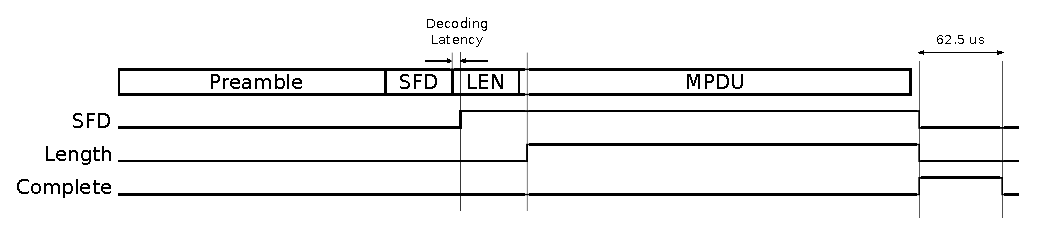
\includegraphics[width=0.96\columnwidth]{pin_activity_rx}
	\caption{Pins activity during receiving}
	\label{fig:pin_activity_rx}
\end{figure}
Since the SmartFusion has PDMA integrated, user can configure the complete as a interrupt to 
processor. Once the complete interrupt arrived, a PDMA transfer unloads the entire packet to
processor.

\subsection{Transmitting}
Similarly, PDMA also benefits the data loading process. User can initiate a PDMA transfer to
load the entire packet into TX fifo. Note that user can start TX transmit without waiting
the DMA transfer completed. Once the TX fifo is empty, a TX complete interrupt asserts.
The signal indicates user is able to load the next packet.
\begin{figure}[h]
\centering
	
\includegraphics[width=0.9\columnwidth]{pin_activity_tx}
	\caption{Interrupts activity during transmitting}
	\label{fig:pin_activity_tx}
\end{figure}
Figure~\ref{fig:pin_activity_tx} shows the interrupts activity. In this example, "Fire" is a MSS GPIO
output which connects to the fabric. User asserts Fire to start transmitting the packet. It is not necessary
to upload the packet before Fire assert. However, data must be start loading before SFD has been transmitted.

\begin{table}[h]
\centering
	\begin{tabular}{|c|c|}
	\end{tabular}
\end{table}
